\documentclass[10pt,aspectratio=169,xcolor=dvipsnames]{beamer}
\usetheme{SimplePlus}
% \setbeameroption{show notes} 

% \setbeameroption{hide notes}
% \setbeameroption{show notes}
% \setbeameroption{show only notes}

\usepackage{graphicx}
\usepackage{graphicx}
\usepackage{subcaption}
\usepackage{xcolor}
\usepackage{comment}
\usepackage{float}
\usepackage{tikz}
\usetikzlibrary{arrows.meta, shapes.geometric, positioning, calc}
\usepackage{pgfplots}
\pgfplotsset{compat=1.18}
\usepackage{amsmath}
\usepackage[french]{babel}
\usepackage[T1]{fontenc}

% Couleurs supplémentaires utiles (les couleurs du thème sont déjà chargées via beamercolorthemeSimplePlus)
\colorlet{MyBlue}{MediumBlue}
\colorlet{MyGreen}{MediumGreen}
\colorlet{MyRed}{MediumRed}

\title{Introduction à l'Optimisation}
\subtitle{Comment les maths trouvent \textit{le meilleur} des mondes ?}
\author{Thibault \and Louis \and Bastien}
\institute{Lamsade}
\date{Février 2026}

\begin{document}

\maketitle

% ============================================================
%  SLIDE : Plan
% ============================================================
% \begin{frame}{Au programme aujourd'hui}
%     \tableofcontents
% \end{frame}

% ============================================================
%  SLIDE : Qui sommes-nous ?
% ============================================================
\begin{frame}{Qui sommes-nous ?}
    \begin{columns}[c]
        \begin{column}{0.3\textwidth}

        
            \begin{block}{\centering Thibault de Surrel}
                \vspace{0.4em}
                \begin{center}
                    \includegraphics[width=2.9cm]{images/thibault2.jpg}
                \end{center}
                \begin{itemize}
                    \item Doctorant 3ème année
                    \item Statistiques
                \end{itemize}
            \end{block}

            
        \end{column}
        \begin{column}{0.3\textwidth}

        
            \begin{block}{\centering Louis}
                \vspace{0.4em}
                \begin{center}
                    \includegraphics[width=2.9cm]{images/louis.jpg}
                \end{center}
                \begin{itemize}
                    \item Doctorant 2ème année
                    \item Recherche opérationnelle
                \end{itemize}
            \end{block}

            
        \end{column}
        \begin{column}{0.3\textwidth}

        
            \begin{block}{\centering Bastien}
                \vspace{0.4em}
                \begin{center}
                    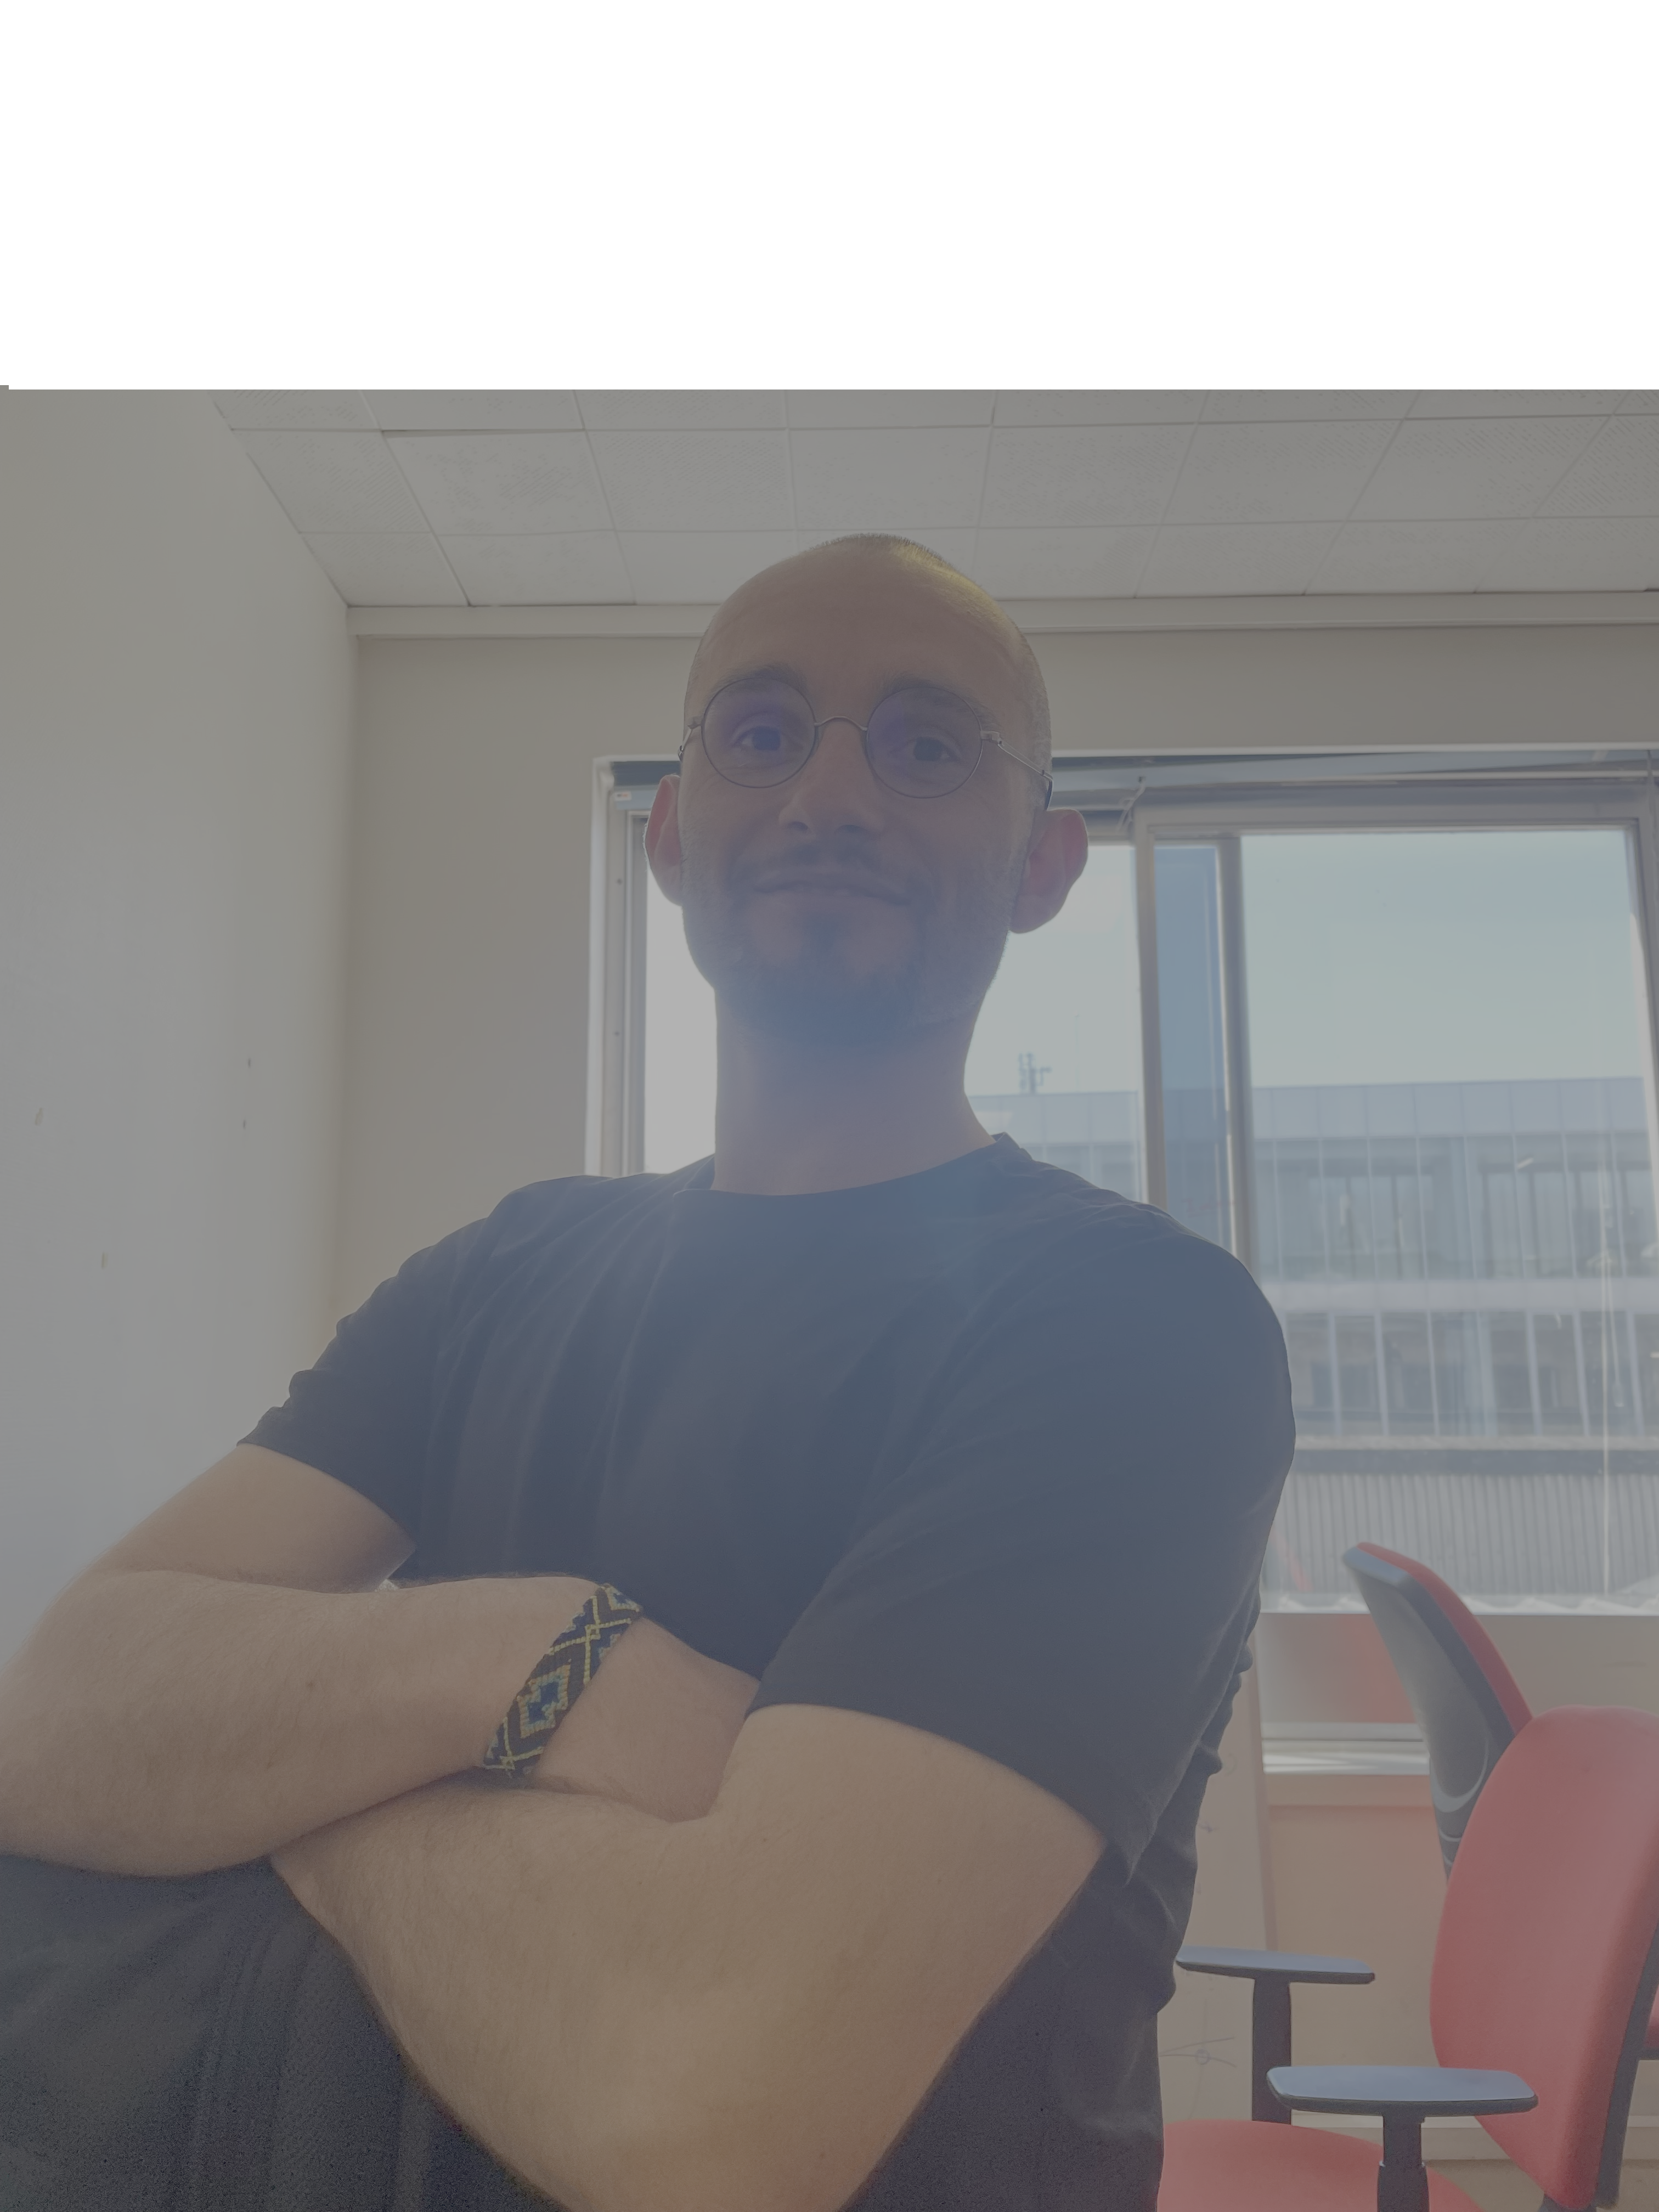
\includegraphics[width=4cm,angle = 270]{images/bastien.jpeg}
                \end{center}
                \begin{itemize}
                    \item Doctorant 2ème année
                    \item Optimisation
                \end{itemize}
            \end{block}

            
        \end{column}
    \end{columns}
\end{frame}

% ============================================================
\section{L'optimisation, c'est quoi ?}
% ============================================================

% ---- Question interactive ----
\begin{frame}{}
    \vspace{1.5em}
    \begin{center}
        {\Large \textbf{Selon vous, qu'est-ce que l'optimisation ?}}
    \end{center}
    \vspace{3em}
    \pause
    \begin{exampleblock}{\centering En un mot\ldots}
        \centering
        L'optimisation, c'est trouver \textbf{le meilleur choix possible} parmi toutes les options.
    \end{exampleblock}
    \vspace{0.5em}
    \pause
    \begin{columns}[c]
        \begin{column}{0.3\textwidth}
            \centering
            \textbf{Minimiser} un coût\\
            \small (argent, électricité, temps\ldots)
        \end{column}
        \begin{column}{0.05\textwidth}
            \centering \large ou
        \end{column}
        \begin{column}{0.3\textwidth}
            \centering
            \textbf{Maximiser} un gain\\
            \small (profit, score à un jeu\ldots)
        \end{column}
        \begin{column}{0.05\textwidth}
            \centering \large $=$
        \end{column}
        \begin{column}{0.25\textwidth}
            \centering
            \textbf{Trouver} le\\
            \textbf{meilleur} $x$
        \end{column}
    \end{columns}
\end{frame}

% ---- Applications ----
\begin{frame}{L'optimisation est partout !}
\begin{figure}[H]
    \centering
    
    % Première ligne
    \onslide<2->{
    \begin{subfigure}{0.32\textwidth}
        \centering
        \includegraphics[width=0.5\linewidth]{images/gps.png}
    \end{subfigure}
    \hfill
    \begin{subfigure}{0.32\textwidth}
        \centering
        \includegraphics[width=\linewidth]{images/netflix.jpg}
    \end{subfigure}
    \hfill
    \begin{subfigure}{0.32\textwidth}
        \centering
        \includegraphics[width=\linewidth]{images/aeronautique1.png}
    \end{subfigure}
    
    \vspace{0.4cm}}
    
    % Deuxième ligne
    \onslide<3->{
    \begin{subfigure}{0.32\textwidth}
        \centering
        \includegraphics[width=\linewidth]{images/medecine.jpeg}
    \end{subfigure}
    \hfill
    \begin{subfigure}{0.32\textwidth}
        \centering
        \includegraphics[width=\linewidth]{images/energie.jpeg}
    \end{subfigure}
    \hfill
    \begin{subfigure}{0.32\textwidth}
        \centering
        \includegraphics[width=0.7\linewidth]{images/IA.png}
    \end{subfigure}}

\end{figure}

\end{frame}

% ---- Lien avec la recherche : boîte noire ----


% ============================================================
\section{Les maths derrière}
% ============================================================

% ---- Qu'est-ce qu'une fonction ? ----
\begin{frame}{Représenter une fonction}
    \centering
            \begin{tikzpicture}
            
                \begin{axis}[
                    width=12cm, height=8cm,
                    xlabel={$x$ \only<2>{\small(paramètre)}},
                    ylabel={$f(x)$ \only<2>{\small(grandeur à optimiser)}},
                    xmin=-3, xmax=3,
                    ymin=0, ymax=5,
                    axis lines=left,
                    grid=major, grid style={gray!25},
                    tick style={draw=none},
                    label style={font=\small},
                    tick label style={font=\tiny},
                    xtick={-2,-1,0,1,2},
                    ytick={1,2,3,4},
                ]
                \addplot[very thick, color=MediumBlue, domain=-3:3, samples=500]
                    {0.5*x^2 + 0.3*sin(deg(4*x)) + 0.8};
                \end{axis}
            \end{tikzpicture}
\end{frame}


% ---- Trouver le minimum à l'oeil : exemple simple ----
\begin{frame}{Où est le minimum ? (1/2)}
    \begin{center}

    \end{center}
    \vspace{0.2em}
    \begin{columns}[c]
        \begin{column}{0.5\textwidth}
            \centering
            \begin{tikzpicture}
                \begin{axis}[
                    width=7cm, height=5cm,
                    xlabel={Température du four (°C)},
                    ylabel={Énergie consommée (kWh)},
                    xmin=100, xmax=300,
                    ymin=0, ymax=4,
                    axis lines=left,
                    grid=major, grid style={gray!25},
                    tick style={draw=none},
                    label style={font=\footnotesize},
                    tick label style={font=\tiny},
                    xtick={100,150,200,250,300},
                    ytick={1,2,3},
                ]
                \addplot[very thick, color=MediumBlue, domain=100:300, samples=100]
                    {0.0003*(x-200)^2 + 0.4};
                \only<2->{\addplot[thin,dashed, color=MediumRed, domain=100:200, samples=500]
                    {+ 0.4};
                \addplot [thin, color = MediumRed] coordinates {(200,0.0) (200,0.4)};}
                
                
                \only<2->{\addplot[mark=*, mark size=  4pt, color=MediumRed]
                    coordinates {(200, 0.4)}
                    node[above,yshift=4pt, font=\small, color=MediumRed] {Minimum !};}
                \end{axis}
            \end{tikzpicture}
        \end{column}
        \begin{column}{0.45\textwidth}
            % \begin{itemize}
            %     \setlength\itemsep{0.5em}
            %     \item On cherche le creux, le point \textbf{le plus bas}
            %     \item Ici : four à 200°C $\Rightarrow$ consommation minimale
            % \end{itemize}
            \begin{center}
            {\large Où est le \textbf{point le plus bas} sur ce graphe ?}\\[0.3em]
            \end{center}
            \vspace{0.5em}
            
            \onslide<2->{\begin{exampleblock}{Réponse}
                Le \textbf{minimum} est en $x^* = 200$°C\\
                avec $f(x^*) = 0{,}4$ kWh.
            \end{exampleblock}}
        \end{column}
    \end{columns}
\end{frame}

% ---- Trouver le minimum à l'oeil : exemple plus dur ----
\begin{frame}{Où est le minimum ? (2/2)}

    \vspace{0.2em}
    \begin{columns}[c]
        \begin{column}{0.5\textwidth}
            \begin{tikzpicture}
                \only<1-2>{\begin{axis}[
                    width=5.2cm, height=7cm,
                    xlabel={$x$},
                    ylabel={$f(x)$},
                    xmin=0, xmax=10,
                    ymin=-3, ymax=4,
                    axis lines=left,
                    grid=major, grid style={gray!25},
                    tick style={draw=none},
                    label style={font=\footnotesize},
                    tick label style={font=\tiny},
                    xtick={0,2,4,6,8,10},
                    ytick={-2,-1,0,1,2,3},
                ]
                \addplot[very thick, color=MediumBlue, domain=0:10, samples=200]
                    {sin(deg(x)) + 0.4*sin(deg(2.5*x)) - 0.15*x + 1.5};
                % local min ~x=4.7
                \only<2->{\addplot[mark=*, mark size=2.5pt, color=orange]
                    coordinates {(4.55, -0.5)}
                    node[below, font=\tiny, color=orange] {minimum ?};
                    \addplot[mark=*, mark size=2.5pt, color=orange]
                    coordinates {(9.8, -0.6)}
                    node[below left, font=\tiny, color=orange] {minimum ?};}
                \end{axis}}
                \only<3>{\begin{axis}[
                    width=7cm, height=7cm,
                    xlabel={$x$},
                    ylabel={$f(x)$},
                    xmin=0, xmax=15,
                    ymin=-3, ymax=4,
                    axis lines=left,
                    grid=major, grid style={gray!25},
                    tick style={draw=none},
                    label style={font=\footnotesize},
                    tick label style={font=\tiny},
                    xtick={0,2,4,6,8,10,12,14},
                    ytick={-2,-1,0,1,2,3},
                ]
                \addplot[very thick, color=MediumBlue, domain=0:15, samples=200]
                    {sin(deg(x)) + 0.4*sin(deg(2.5*x)) - 0.15*x + 1.5};
                % local min ~x=4.7
                \addplot[mark=*, mark size=2.5pt, color=orange]
                    coordinates {(4.55, -0.5)}
                    node[below, font=\tiny, color=orange] {minimum ?};
                % global min ~x=8.2
                \addplot[mark=*, mark size=3.5pt, color=MediumRed]
                    coordinates {(11.7, -1.35)}
                    node[below, font=\small, color=MediumRed] {vrai minimum !};
\end{axis}}
            \end{tikzpicture}


        \end{column}
        \begin{column}{0.45\textwidth}
                \begin{center}
                    {\large Et maintenant ? Repérez le \textbf{minimum} !}
                \end{center}

            \vspace{0.4em}
            \onslide<3->{
            \begin{alertblock}{Piège !}
                On peut se tromper de minimum.\\
                C'est un des grands défis de l'optimisation !
            \end{alertblock}}
        \end{column}
    \end{columns}
\end{frame}

\begin{frame}{Traduire un problème de la vraie vie en maths ("modéliser")}
\begin{exampleblock}{
    Un producteur de poire observe:}
    \begin{itemize}
        \item s'il y a 60 poiriers sur son champs, chaque arbre produit 480 poires par an.
        \item à chaque fois qu'un poirier est ajouté, tous les poiriers produisent 5 poires de moins.
    \end{itemize}
    Combien doit-il planter d'arbre pour produire le plus de poires ?
\end{exampleblock}
\onslide<2->{
\begin{exampleblock}{Recette}
    \begin{itemize}
        \item Si on ajoute $1$ poirier : $(480-5\times 1)\times(60+1)$ poires produites.
        \onslide<3->{
        \newline Si on ajoute $2$ poirier : $(480-5\times 2)\times(60+2)$ poires produites.}
        \onslide<4->{
        \newline Si on ajoute $p$ poirier : \textcolor{blue}{$(480-5\times p)\times(60+p)$} poires produites.}
        \onslide<5>{
        \item La nouvelle question est : \newline
        \vspace{0.5em}   \flqq{} Quel est le point le \textbf{plus haut} de la fonction \textcolor{blue}{$f(p)=(480-5\times p)\times(60+p)$ ?\frqq{}}} 
    \end{itemize}
\end{exampleblock}}
\end{frame}

\begin{frame}{Représentation graphique du nombre de poires produites}
\centering
    
                \begin{tikzpicture}
                \begin{axis}[
                    width=10cm, height=8cm,
                    xlabel={$p$  (poiriers plantés)},
                    ylabel={$f(p)$ (poires/an)},
                    xmin=0, xmax=60,
                    ymin=23000, ymax=33000,
                    axis lines=left,
                    grid=major, grid style={gray!25},
                    tick style={draw=none},
                    label style={font=\small},
                    tick label style={font=\tiny},
                    xtick={0,10,20,30,40,50,60},
                    ytick={23000,24000, 25000, 26000,27000, 28000,29000, 30000,31000,32000},
                    scaled y ticks=false,
                ]
                \addplot[very thick, color=MediumBlue, domain=0:60, samples=500]
                    {(480-5*x)*(60+x)};



                \only<2->{\addplot[thin, color=MediumRed, domain=0:18, samples=500]
                    {+ 30420};
                \addplot [thin, color = MediumRed] coordinates {(18,0) (18, 30420)};
                
                \addplot[mark=*, mark size=  4pt, color=MediumRed]
                    coordinates {(18, 30420)}
                    node[above right, font=\small, color=MediumRed] {Maximum atteint en $p=18$!};}

                    
                \end{axis}
            \end{tikzpicture}
    
\end{frame}


% ---- Pourquoi des algorithmes ? ----
\begin{frame}{Pourquoi on a besoin d'algorithmes ?}
    \begin{columns}[c]
        \begin{column}{0.55\textwidth}
            \begin{figure}
                \centering
                \includegraphics[width=0.8\linewidth]{optimlandscape.jpg}
                \caption*{Plusieurs paramètres (latitude \& longitude)}
            \end{figure}
        \end{column}
        \begin{column}{0.42\textwidth}
            \begin{alertblock}{Le problème}
                Imaginez : vous êtes dans un paysage de montagnes et de vallées,\\[0.3em]
                \textbf{les yeux bandés}.\\[0.3em]
                Comment trouver le point le plus bas ?
            \end{alertblock}
            \vspace{0.5em}
            \pause
            \begin{exampleblock}{La solution}
                Des \textbf{algorithmes} qui explorent intelligemment le paysage.
            \end{exampleblock}
        \end{column}
    \end{columns}
\end{frame}


% ---- Suivre la pente ----
\begin{frame}{L'intuition : suivre la pente}
    \begin{columns}[c]
        \begin{column}{0.5\textwidth}
            \textbf{Imaginez une balle au sommet d'une colline\ldots}
            \vspace{0.5em}
            % \begin{itemize}
            %     \setlength\itemsep{0.5em}
            %     \item Elle roule toujours \textbf{vers le bas}
            %     \item À chaque instant, elle suit la \textbf{direction de la pente}
            %     \item Elle finit par s'arrêter dans un creux
            % \end{itemize}
            \vspace{0.5em}
            \onslide<4->{
            \begin{block}{Descente de \emph{gradient}}
                À chaque étape : faire un \textbf{pas dans la direction descendante}.
            \end{block}}

            % \onslide<6->{\begin{alertblock}{Attention}
            %     Si le pas est trop grand, on s'éloigne du minimum
            % \end{alertblock}}
        \end{column}
        \begin{column}{0.47\textwidth}
            \centering
            \begin{tikzpicture}
            \only<1-4>{                \begin{axis}[
                    width=6.5cm, height=5.5cm,
                    xmin=-3.2, xmax=3.2, ymin=-0.2, ymax=6,
                    axis lines=left,
                    tick style={draw=none},
                    xtick=\empty, ytick=\empty,
                    xlabel={$x$}, ylabel={$f(x)$},
                    label style={font=\small},
                ]
                \addplot[thick, color=MediumBlue, domain=-3:3, samples=100]
                    {0.6*x^2 + 0.3};
                % Points de la descente
                \only<1->{
                \addplot[mark=*, mark size=4.5pt, color=MediumRed]
                    coordinates {(-2.7, 4.67)};
                \node[color=MediumRed, font=\scriptsize]
                    at (axis cs:-2.3, 5.3) {départ};}
                \only<2->{
                \draw[->, thick, color=MediumRed!80]
                    (axis cs:-2.7, 4.67) -- (axis cs:-1.8, 2.25);
                \addplot[mark=*, mark size=4pt, color=orange]
                    coordinates {(-1.7, 2.03)};}
                \only<3->{    
                \draw[->, thick, color=orange!90]
                    (axis cs:-1.7, 2.03) -- (axis cs:-0.8, 0.7);
                \addplot[mark=*, mark size=3.5pt, color=MediumGreen]
                    coordinates {(-0.7, 0.59)};}
                \only<4->{
                \draw[->, thick, color=MediumGreen!80]
                    (axis cs:-0.7, 0.59) -- (axis cs:-0.1, 0.35);
                \addplot[mark=*, mark size=3.5pt, color=MediumGreen]
                    coordinates {(0, 0.3)};
                \node[color=MediumGreen, font=\scriptsize]
                    at (axis cs:1.1, 0.2) {arrivée !};}
                \end{axis}
}
            % \only<5->{                \begin{axis}[
                    width=6.5cm, height=5.5cm,
                    xmin=-3.2, xmax=3.2, ymin=-0.2, ymax=6,
                    axis lines=left,
                    tick style={draw=none},
                    xtick=\empty, ytick=\empty,
                    xlabel={$x$}, ylabel={$f(x)$},
                    label style={font=\small},
                ]
                \addplot[thick, color=MediumBlue, domain=-3:3, samples=100]
                    {0.6*x^2 + 0.3};
                % Points de la descente
                {
                \addplot[mark=*, mark size=4.5pt, color=MediumRed]
                    coordinates {(-2.7, 4.67)};
                \node[color=MediumRed, font=\scriptsize]
                    at (axis cs:-2.3, 5.3) {départ};}
                {
                \draw[->, thick, color=MediumRed!80]
                    (axis cs:-2.7, 4.67) -- (axis cs:-1.7,2.03);
                \addplot[mark=*, mark size=4pt, color=orange]
                    coordinates {(-1.7, 2.03)};}
                \only<6->{    
                \draw[->, thick, color=orange!90]
                    (axis cs:-1.7, 2.03) -- (axis cs:2.,3.);
                \node[color=orange!90, font=\scriptsize]
                    at (axis cs:1., 3.3) {grand pas};
                \addplot[mark=*, mark size=3.5pt, color=MediumGreen]
                    coordinates {(2.12, 3)};}
                \end{axis}}
            \end{tikzpicture}
        \end{column}
    \end{columns}
\end{frame}

\begin{frame}{Et quand on ne voit pas la pente ? La \emph{boîte noire.}}
            \textbf{Exemple 1:} trouver la meilleure dose d'un médicament.
            \vspace{0.5em}


            \centering
            \begin{tikzpicture}[node distance=0.8cm, >=Stealth]
                \node[draw, thick, rounded corners=6pt,
                      minimum width=3.5cm, minimum height=2cm,
                      fill=MutedBlue, font=\bfseries] (box) {Boîte noire};
                \node[left=1.2cm of box, font=\small] (in) {dose $x$};
                \node[right=1.2cm of box, font=\small] (out) {effet $f(x)$};
                \draw[->, thick] (in) -- (box);
                \draw[->, thick] (box) -- (out);
                \node[below=0.3cm of box, font=\small\itshape,
                      text=gray, align=center] {On ne sait pas ce\\qu'il y a dedans !};
            \end{tikzpicture}

            \begin{alertblock}{Le problème}
                On ne peut pas \textbf{calculer la pente} de cette boîte noire.\\
                $\Rightarrow$ Comment trouver la meilleure dose quand même ?
            \end{alertblock}
\end{frame}

% ============================================================
\section{Comment chercher sans voir ?}
% ============================================================



% ---- Contre-exemple : sonder un lac ----
\begin{frame}{Autre exemple de boîte noire}
    \begin{columns}[c]
        \begin{column}{0.5\textwidth}
            \textbf{Mission : trouver l'endroit le plus profond d'un lac.}
            
            \vspace{0.5em}
            
            \begin{alertblock}{Problème}
                On ne peut \textbf{pas} mesurer la pente.
            \end{alertblock}
            \onslide<2->{
            \begin{exampleblock}{Stratégie}
                Regarder à droite, à gauche de l'endroit sondé.
            \end{exampleblock}}
        \end{column}
        \begin{column}{0.47\textwidth}
            \centering
            \begin{tikzpicture}[scale=0.85]
                % % Eau
                % \fill[cyan!15] (0,2.2) rectangle (6, 3.5);
                \draw[thick, cyan!50] (0,3) -- (6,3);
                \node[font=\footnotesize, color=cyan!60!black, anchor=west]
                    at (0.2, 3.25) {Surface};
                % % Fond
                % \fill[brown!25]
                %     (0,0) -- (0,1.2)
                %     .. controls (1,2) and (1.5,0.5) .. (2.5,0.1)
                %     .. controls (3.5,-0.4) and (4,0.5) .. (5,1.5)
                %     -- (6,1.8) -- (6,0) -- cycle;
                % \draw[thick, brown!70]
                %     (0,1.2)
                %     .. controls (1,2) and (1.5,0.5) .. (2.5,0.1)
                %     .. controls (3.5,-0.4) and (4,0.5) .. (5,1.5);
                % % Sonde
                % \draw[very thick, gray] (1.5, 3) -- (1.5, 1.7);
                % \fill[gray!70] (1.5, 1.7) circle (3.5pt);
                % \node[font=\tiny, above] at (1.5, 3.1) {sonde};
                % % Annotation profondeur
                % \draw[<->, thick, MediumRed] (3.2, 3) -- (3.2, 0.1);
                % \node[font=\tiny, color=MediumRed, right] at (3.3, 1.5) {profondeur};
                % \node[font=\tiny, color=MediumRed, right] at (3.3, 0.1) {$\leftarrow$ minimum ?};

                % Eau
\fill[cyan!15]
    (0,3.5) -- (0,1.2)
    .. controls (1,2) and (1.5,0.5) .. (2.5,0.1)
    .. controls (3.5,-0.4) and (4,0.5) .. (5,1.5)
    -- (6,1.8) -- (6,3.5) -- cycle;

\draw[thick, cyan!50] (0,3) -- (6,3);
\node[font=\footnotesize, color=cyan!60!black, anchor=west]
    at (4.5, 3.25) {Surface};
    
% Fond
\fill[brown!25]
    (0,-0.5) -- (0,1.2)
    .. controls (1,2) and (1.5,0.5) .. (2.5,0.1)
    .. controls (3.5,-0.4) and (4,0.5) .. (5,1.5)
    -- (6,1.8) -- (6,-0.5) -- cycle;
\draw[thick, brown!70]
    (0,1.2)
    .. controls (1,2) and (1.5,0.5) .. (2.5,0.1)
    .. controls (3.5,-0.4) and (4,0.5) .. (5,1.5) -- (6,1.8);
% Sonde
\draw[very thick, gray] (1.5, 3) -- (1.5, 0.9);
\fill[gray!70] (1.5, 0.9) circle (3.5pt);
\node[font=\footnotesize, left] at (1.5, 0.9) {sonde};
% Annotation profondeur
\draw[<->, thick, MediumRed] (3.0, 3) -- (3.0, 0.1);
\node[font=\footnotesize, color=MediumRed, below right] at (3.0, 0.0) {profondeur max.};



\begin{scope}[shift = {(1.,3.6)},scale = 0.25]
    \draw[thick] (0,0) arc[start angle=180,end angle=360,radius=2];
  \draw (0,0) -- (4,0) ;
  \draw (2,0.) -- (2,3); % mast
  \draw (2,3) -- (4,1)--(2,1); % sail
  \fill[MediumGreen] (2,3) -- (4,1)--(2,1) -- cycle;
\end{scope}











% % Surface de l'eau
% \draw[thick, cyan!50] (0,3) -- (6,3);

% % Eau (épouse exactement la forme du fond)
% \fill[cyan!15]
%     (0,3) -- (0,1.2)
%     .. controls (1,2) and (1.5,0.5) .. (2.5,0.1)
%     .. controls (3.5,-0.4) and (4,0.5) .. (5,1.5)
%     -- (6,1.8) -- (6,3) -- cycle;

% % Fond
% \fill[brown!25]
%     (0,0) -- (0,1.2)
%     .. controls (1,2) and (1.5,0.5) .. (2.5,0.1)
%     .. controls (3.5,-0.4) and (4,0.5) .. (5,1.5)
%     -- (6,1.8)

            \end{tikzpicture}
        \end{column}
    \end{columns}
\end{frame}

% ---- La notion de pas ----
\begin{frame}{La notion de pas}
    % \begin{columns}[c]
    %     \begin{column}{0.45\textwidth}
    %         \begin{itemize}
    %             \setlength\itemsep{0.6em}
    %             \item On \textbf{sonde} des points autour de nous
    %             \item On se déplace vers le point le plus intéressant
    %             \item La \textbf{taille du pas} est cruciale :
    %                 \begin{itemize}
    %                     \setlength\itemsep{0.3em}
    %                     \item Trop grand $\Rightarrow$ on rate le minimum
    %                     \item Trop petit $\Rightarrow$ on est trop lent
    %                 \end{itemize}
    %         \end{itemize}
    %         \vspace{0.5em}

    %     \end{column}
    %     \begin{column}{0.52\textwidth}
    %         \centering
    %         \begin{tikzpicture}
    %             \begin{axis}[
                    width=7.5cm, height=5.5cm,
                    xmin=0, xmax=6, ymin=-0.5, ymax=4,
                    axis lines=left,
                    tick style={draw=none},
                    xtick=\empty, ytick=\empty,
                    xlabel={$x$}, ylabel={$f(x)$},
                    label style={font=\small},
                ]
                \addplot[thick, color=MediumBlue, domain=0:6, samples=150]
                    {0.5*(x-3)^2 + 0.3};
                % Grand pas (rate)
                \addplot[mark=*, mark size=3.5pt, color=MediumRed]
                    coordinates {(0.4, 3.6)};
                \addplot[mark=*, mark size=3.5pt, color=MediumRed]
                    coordinates {(5.5, 3.45)};
                \draw[<->, dashed, MediumRed, thick]
                    (axis cs:0.3, 2.3) -- (axis cs:5.7, 2.3)
                    node[midway, above, font=\small, color=MediumRed] {pas trop grand};
                % Petit pas (adapté)
                \addplot[mark=*, mark size=3.5pt, color=MediumGreen]
                    coordinates {(1.8, 1.)};
                \addplot[mark=*, mark size=3.5pt, color=gray]
                    coordinates {(2.4, 0.48)};
                \addplot[mark=*, mark size=3.5pt, color=MediumGreen]
                    coordinates {(3.0, 0.3)};
                \draw[<->, dashed, MediumGreen, thick]
                    (axis cs:1.8, 0.05) -- (axis cs:3.0, 0.05)
                    node[midway, below, font=\small, color=MediumGreen] {pas adapté};
                \end{axis}
    %         \end{tikzpicture}
    %     \end{column}
    % \end{columns}
    \centering
    
    \begin{tikzpicture}
    \begin{axis}[
                    width=7.5cm, height=5.5cm,
                    xmin=0, xmax=6, ymin=-0.5, ymax=4,
                    axis lines=left,
                    tick style={draw=none},
                    xtick=\empty, ytick=\empty,
                    xlabel={$x$}, ylabel={$f(x)$},
                    label style={font=\small},
                ]
                \addplot[thick, color=MediumBlue, domain=0:6, samples=150]
                    {0.5*(x-3)^2 + 0.3};
                % Grand pas (rate)
                \addplot[mark=*, mark size=3.5pt, color=MediumRed]
                    coordinates {(0.4, 3.6)};
                \addplot[mark=*, mark size=3.5pt, color=MediumRed]
                    coordinates {(5.5, 3.45)};
                \draw[<->, dashed, MediumRed, thick]
                    (axis cs:0.3, 2.3) -- (axis cs:5.7, 2.3)
                    node[midway, above, font=\small, color=MediumRed] {pas trop grand};
                % Petit pas (adapté)
                \addplot[mark=*, mark size=3.5pt, color=MediumGreen]
                    coordinates {(1.8, 1.)};
                \addplot[mark=*, mark size=3.5pt, color=gray]
                    coordinates {(2.4, 0.48)};
                \addplot[mark=*, mark size=3.5pt, color=MediumGreen]
                    coordinates {(3.0, 0.3)};
                \draw[<->, dashed, MediumGreen, thick]
                    (axis cs:1.8, 0.05) -- (axis cs:3.0, 0.05)
                    node[midway, below, font=\small, color=MediumGreen] {pas adapté};
                \end{axis}
    \end{tikzpicture}
\end{frame}

% ============================================================
\section{Votre mission : la tortue !}
% ============================================================

% ---- La mission ----
\begin{frame}{Votre mission}
    \begin{columns}[c]
        \begin{column}{0.52\textwidth}
            \begin{block}{Contexte}
                Les tortues marines pondent leurs œufs sur la plage.\\[0.4em]
                Notre tortue cherche l'\textbf{endroit le plus frais} pour le bon développement des bébé tortues.
            \end{block}
            \vspace{0.4em}
            \begin{exampleblock}{Votre rôle}
                Vous êtes la tortue !\\[0.3em]
                Rejoignez l'endroit de \textbf{température minimale}
            \end{exampleblock}
        \end{column}
        \begin{column}{0.45\textwidth}
            \begin{figure}
                \centering
                \includegraphics[width=0.8\linewidth]{images/tortue.png}
            \end{figure}
        \end{column}
    \end{columns}
\end{frame}

% ---- Faire le lien avec l'optimisation ----
\begin{frame}{Le lien avec l'optimisation}
    \begin{center}
        \begin{tikzpicture}[node distance=0.5cm, >=Stealth]
            \node[draw, rounded corners=6pt,
                  fill=MutedBlue, minimum width=3.8cm, minimum height=1.6cm,
                  font=\small, align=center] (a) at (-4.5, 0)
                {\textbf{Paramètre $x$}\\[0.2em] position de la tortue\\(latitude, longitude)};
            \node[draw, rounded corners=6pt,
                  fill=MutedGreen, minimum width=3.8cm, minimum height=1.6cm,
                  font=\small, align=center] (b) at (0, 0)
                {\textbf{Fonction $f(x)$}\\[0.2em] température du sable\\à la position $x$};
            \node[draw, rounded corners=6pt,
                  fill=MutedRed, minimum width=3.8cm, minimum height=1.6cm,
                  font=\small, align=center] (c) at (4.5, 0)
                {\textbf{Minimum $x^*$}\\[0.2em] l'endroit\\le plus frais !};
            \draw[->, very thick] (a) -- (b);
            \draw[->, very thick] (b) -- (c);
        \end{tikzpicture}
    \end{center}
    \vspace{0.5em}
    \begin{columns}[c]
        \begin{column}{0.48\textwidth}
            \begin{block}{Règles du jeu}
                \begin{itemize}
                    \item Vous pouvez \textbf{sonder} la température à plusieurs endroits
                    \item Vous avez un nombre \textbf{limité de sondes}
                    \item Objectif : trouver le minimum \textbf{en un minimum d'essais}
                \end{itemize}
            \end{block}
        \end{column}
        \begin{column}{0.48\textwidth}
            \begin{alertblock}{Contrainte}
                Vous ne voyez pas la carte de chaleur complète.\\[0.3em]
                Vous ne mesurez la température qu'aux points où vous envoyez la tortue.\\[0.3em]
            \end{alertblock}
        \end{column}
    \end{columns}
\end{frame}

% ---- A vous de jouer ----
\begin{frame}{A vous de jouer !}
\begin{figure}
    \centering
    \includegraphics[width=\linewidth]{images/tortuebis.jpg}
\end{figure}
\end{frame}

\end{document}
